% ST4001 Senior Thesis draft.
% Compile with XeLaTeX or LuaLaTeX.
\documentclass[12pt,a4paper]{report}

\usepackage[a4paper,left=1in,right=1in,top=1in,bottom=1in]{geometry}
\usepackage{fontspec}
\usepackage{setspace}
\usepackage{fancyhdr}
\usepackage{titlesec}
\usepackage{tocloft}
\usepackage{graphicx}
\usepackage{booktabs}
\usepackage{array}
\usepackage{longtable}
\usepackage{tabularx}
\usepackage{amsmath,amssymb}
\usepackage{caption}
\usepackage{enumitem}
\usepackage[hidelinks]{hyperref}

\setmainfont{Times New Roman}
\doublespacing
\setlength{\parindent}{2em}
\setlength{\parskip}{0pt}

\newcommand{\ThesisTitle}{Transformer-Based Low-Dose CT Image Denoising with Residual Noise Analysis}
\newcommand{\StudentName}{Your Name}
\newcommand{\StudentID}{Your student ID}
\newcommand{\SupervisorName}{Supervisor Name}
\newcommand{\SupervisorTitle}{Academic Title}
\newcommand{\ClassYear}{Class of 2026}
\newcommand{\Major}{Your Major}
\newcommand{\SubmissionDate}{June 2026}
\renewcommand{\bibname}{References}

\pagestyle{fancy}
\fancyhf{}
\fancyhead[L]{\ClassYear}
\fancyhead[C]{\StudentName}
\fancyhead[R]{\StudentID}
\fancyfoot[C]{\thepage}
\renewcommand{\headrulewidth}{0pt}

\titleformat{\chapter}[block]
  {\normalfont\bfseries\fontsize{18}{22}\selectfont}
  {Chapter \thechapter.}{0.75em}{}
\titlespacing*{\chapter}{0pt}{0pt}{18pt}
\titleformat{\section}
  {\normalfont\bfseries\fontsize{14}{18}\selectfont}
  {\thesection}{0.75em}{}
\titleformat{\subsection}
  {\normalfont\bfseries\fontsize{12}{16}\selectfont}
  {\thesubsection}{0.75em}{}

\captionsetup[figure]{font={bf,small},labelfont=bf,justification=centering,singlelinecheck=true}
\captionsetup[table]{font={bf,small},labelfont=bf,justification=centering,singlelinecheck=true}

\newcommand{\fronttitle}[1]{%
  \clearpage
  \begin{center}
    {\bfseries\fontsize{24}{28}\selectfont #1}
  \end{center}
  \vspace{1em}
}

\newcommand{\signatureline}[1]{%
  \noindent #1\hspace{0.5em}\rule{0.32\textwidth}{0.4pt}
}

\begin{document}

\begin{titlepage}
\thispagestyle{empty}
\begin{flushright}
Confidential thesis $\square$
\end{flushright}
\vspace*{1.2cm}
\begin{center}
{\fontsize{18}{22}\selectfont Zhejiang University-University of Illinois Urbana-Champaign Institute\par}
\vspace{1.4cm}
{\bfseries\fontsize{24}{30}\selectfont Undergraduate Thesis\par}
\vspace{0.3cm}
{\bfseries\fontsize{20}{24}\selectfont (Design)\par}
\vspace{2.2cm}
{\bfseries\fontsize{20}{24}\selectfont \ThesisTitle\par}
\vfill
\renewcommand{\arraystretch}{1.6}
\begin{tabular}{>{\raggedleft\arraybackslash}p{0.28\textwidth} p{0.45\textwidth}}
Student Name & \StudentName\\
Student ID & \StudentID\\
Supervisor & \SupervisorName\\
Class of year & \ClassYear\\
Major & \Major\\
Submission date & \SubmissionDate\\
\end{tabular}
\end{center}
\end{titlepage}

\setcounter{page}{2}

\fronttitle{Content Checklist}

\begin{center}
\small
(Student should bind this form on the first page of the thesis after the cover page. The form should be filled out by the supervisor after the oral defense.)
\end{center}
\vspace{0.5em}

\renewcommand{\arraystretch}{1.35}
\begin{tabularx}{\textwidth}{|p{0.18\textwidth}|X|p{0.18\textwidth}|X|}
\hline
Student Name & \StudentName & ZJU ID & \StudentID\\ \hline
Major & \Major & Academic Supervisor Title & \SupervisorTitle\\ \hline
Thesis title & \multicolumn{3}{p{0.69\textwidth}|}{\ThesisTitle}\\ \hline
Evaluation & \multicolumn{3}{p{0.69\textwidth}|}{Good $\square$\quad Fair $\square$}\\ \hline
\end{tabularx}

\vspace{1em}
\begin{longtable}{|c|p{0.68\textwidth}|c|}
\hline
 & Content Checklist Section & $\sqrt{}$ \\ \hline
1 & Cover (Use the unified cover, blue recommended) & \\ \hline
2 & Academic Integrity Commitment of Senior Thesis & \\ \hline
3 & Acknowledgements & \\ \hline
4 & Abstract & \\ \hline
5 & Table of Contents & \\ \hline
6 & Main Content (Page numbers start from the main text) & \\ \hline
7 & Reference & \\ \hline
8 & Appendix (if need) & \\ \hline
9 & Author's Biography & \\ \hline
10 & Task plan of senior thesis & \\ \hline
11 & Assessment Form of senior thesis & \\ \hline
12 & On-site Minutes Form of Oral Defense & \\ \hline
\end{longtable}

\vspace{2em}
\signatureline{Signature of Supervisor:}
\hfill
\signatureline{Date:}

\fronttitle{Academic Integrity Commitment of Senior Thesis}

\begin{enumerate}[leftmargin=*,label=\arabic*.]
\item I solemnly promise that the submitted thesis has been completed under the guidance of my supervisor in strict accordance with the relevant regulations of the university and the college.
\item In my thesis, except for the parts specifically marked and acknowledged, it does not contain research results that have been published or written by others, nor does it contain materials used to obtain degrees or certificates from Zhejiang University or other educational institutions.
\item Any contributions made by my colleagues to this research have been clearly stated and acknowledged in the thesis.
\item I promise that there has been no fabrication of data in the process of completing the thesis.
\item If there is any infringement of intellectual property rights in this thesis, I shall bear the corresponding legal responsibilities.
\item I fully understand that Zhejiang University has the right to retain and submit copies and disks of this thesis (design) to relevant departments or agencies, and to allow the thesis (design) to be consulted and borrowed. I authorize Zhejiang University to include all or part of this thesis (design) in relevant databases for retrieval and dissemination, and to save and compile this thesis (design) by means of photocopying, reduction, or scanning.
\end{enumerate}

\vspace{3em}
\signatureline{Author's Signature:}
\hfill
\signatureline{Supervisor's Signature:}

\vspace{2em}
\signatureline{Date:}
\hfill
\signatureline{Date:}

\fronttitle{Acknowledgements}

I would like to express my sincere gratitude to my supervisor for guidance, feedback, and support throughout this senior thesis project. I also thank the ZJU-UIUC Institute for providing the academic environment and project framework for this work. Finally, I thank my classmates, friends, and family for their encouragement during the implementation, debugging, training, and writing stages of this project.

\fronttitle{Abstract}

Low-dose computed tomography (LDCT) reduces ionizing radiation exposure but introduces stronger quantum noise and artifacts that may obscure anatomical details. This thesis studies LDCT denoising as a supervised image restoration problem using paired quarter-dose and full-dose CT slices. The main objective is to implement and evaluate Transformer-based denoising models, with RED-CNN and CTformer as baselines and a Restormer-style model, named CTRestormer, as the main experimental model. Experiments are conducted on a prepared AAPM-Mayo 3mm B30 dataset using a held-out patient split. Peak signal-to-noise ratio (PSNR), structural similarity (SSIM), and root mean square error (RMSE) are used for quantitative evaluation, while qualitative images and residual noise maps are proposed for structural analysis. The original low-dose input achieves 29.2489 dB PSNR, 0.8759 SSIM, and 14.2416 RMSE on the held-out L506 patient. After fine-tuning, CTRestormer at 21,500 iterations achieves 32.6738 dB PSNR, 0.9096 SSIM, and 9.4842 RMSE, slightly exceeding the reproduced CTformer and RED-CNN baselines. These results show that a resource-adapted Transformer restoration model can effectively denoise LDCT images and become competitive after careful training. The thesis further argues that numerical metrics alone are insufficient for medical denoising, and proposes residual noise, noise texture, edge preservation, and Noise2Noise-style experiments as extensions to evaluate whether models remove noise without suppressing diagnostically relevant structures.

\noindent\textbf{Keywords:} Low-dose CT; medical image denoising; image restoration; Transformer; Restormer; CTformer; RED-CNN; residual noise analysis.

\clearpage
\begin{center}
{\bfseries\fontsize{24}{28}\selectfont Content}
\end{center}
\renewcommand{\contentsname}{}
\tableofcontents

\clearpage
\setcounter{page}{1}

\chapter{Introduction}

Computed tomography (CT) is one of the most important imaging modalities in modern clinical practice. It provides cross-sectional information about internal anatomical structures and is widely used for screening, diagnosis, treatment planning, and follow-up examinations. However, CT imaging relies on ionizing radiation. Although a single scan is usually clinically justified, repeated examinations and scans for vulnerable populations raise concerns about cumulative radiation exposure. Reducing radiation dose is therefore an important goal in medical imaging.

The direct consequence of lowering radiation dose is image degradation. In low-dose CT, fewer photons contribute to the measurement process, and the reconstructed image usually contains stronger quantum noise, streak-like artifacts, and reduced low-contrast visibility. These artifacts can make soft tissue boundaries less clear and can reduce confidence in small or subtle findings. Therefore, the technical challenge is not only to make an image appear smoother, but to suppress noise while preserving true anatomical structures.

LDCT denoising can be formulated as an image restoration problem. Given a low-dose image, the algorithm estimates an image that is close to the corresponding normal-dose or full-dose image. Traditional methods use handcrafted priors, non-local similarity, dictionary learning, total variation, or iterative reconstruction. These approaches are useful but may require careful parameter tuning and may not fully capture spatially varying noise patterns.

Deep learning provides a data-driven alternative. With paired low-dose and full-dose CT data, a neural network can learn the mapping from noisy images to cleaner references. Convolutional neural networks (CNNs), especially encoder-decoder and residual architectures, have been widely used for this task. RED-CNN is a representative LDCT denoising model and remains a strong baseline. More recently, Transformer-based image restoration models have become attractive because self-attention can model broader contextual dependencies than local convolution alone.

This thesis focuses on Transformer-based LDCT denoising under practical local hardware constraints. The project begins with a reproduction and evaluation of CTformer, a convolution-free Token2Token dilated vision Transformer for LDCT denoising. RED-CNN is used as a classic CNN baseline. The main experimental model is CTRestormer, a Restormer-inspired hierarchical Transformer adapted for the 3mm B30 AAPM-Mayo dataset and a 6GB NVIDIA RTX 3060 Laptop GPU. The study evaluates whether this Transformer restoration model can improve over both the low-dose input and existing baselines.

The current experiments show that all learned models improve substantially over the low-dose input. More importantly, after fine-tuning, CTRestormer reaches 32.6738 dB PSNR and 0.9096 SSIM on the held-out L506 patient, slightly exceeding the reproduced CTformer and RED-CNN baselines. This result supports the value of Transformer restoration for LDCT denoising. At the same time, the small numerical margin makes further analysis necessary. A denoising model can improve PSNR by oversmoothing, so residual noise maps and noise texture analysis are proposed to examine what each model removes from the input.

\section{Research Objectives}

The objectives of this thesis are:

\begin{enumerate}[leftmargin=*]
\item To implement and organize LDCT denoising experiments using CTformer, RED-CNN, and a Restormer-style Transformer model.
\item To evaluate models on a patient-level held-out test split using PSNR, SSIM, and RMSE.
\item To analyze training behavior and checkpoint-level performance, especially for CTRestormer fine-tuning.
\item To propose residual noise map and Noise2Noise-style experiments that can reveal whether denoising models remove true noise or suppress anatomical details.
\item To produce a reproducible thesis workflow that can be extended with additional experiments before final submission.
\end{enumerate}

\section{Thesis Organization}

Chapter 2 reviews LDCT denoising and related CNN and Transformer models. Chapter 3 describes the methodology, including problem formulation, model architectures, losses, and residual noise analysis. Chapter 4 presents the experimental setup. Chapter 5 reports current quantitative and qualitative results. Chapter 6 discusses extended experiments and future improvements. Chapter 7 concludes the thesis.

\chapter{Literature Review}

\section{Low-Dose CT Denoising}

The AAPM-Mayo Low Dose CT Grand Challenge is a widely used benchmark for LDCT research. It provides paired normal-dose and simulated quarter-dose CT images, making supervised learning possible. In this setting, the low-dose image is used as input and the full-dose image is used as the target. Although full-dose CT is not perfectly noise-free, it is a clinically meaningful reference for restoration.

LDCT denoising differs from ordinary natural image denoising in several ways. First, CT intensity values have physical meaning and are related to tissue attenuation. Second, subtle structures can be diagnostically important, so excessive smoothing may be harmful. Third, CT noise texture is not only visual noise; it is affected by acquisition geometry, reconstruction kernel, dose level, and slice thickness. A denoising method should therefore preserve structural information while reducing noise in a controlled manner.

Standard quantitative metrics include PSNR, SSIM, and RMSE. PSNR and RMSE measure pixel-level fidelity, while SSIM measures structural similarity. These metrics are useful for benchmarking but incomplete for clinical evaluation. A model with high PSNR may still erase low-contrast details. For this reason, residual maps, edge preservation measures, and noise texture analysis are important complements.

\section{CNN-Based Image Restoration}

CNNs are natural candidates for image restoration because convolution is well matched to local spatial patterns. U-Net introduced a multi-scale encoder-decoder architecture with skip connections for biomedical image segmentation, and the same structure has been widely adapted to restoration. In denoising, encoder layers extract features at multiple scales, while decoder layers reconstruct an image aligned with the input.

RED-CNN is a representative LDCT denoising method. It uses residual encoder-decoder convolutional layers to learn a correction from low-dose to normal-dose CT. The residual formulation is especially suitable because the low-dose image already contains most anatomical content. The network does not need to generate a new image from scratch; instead, it learns to remove noise and artifacts while preserving anatomy. RED-CNN is compact, stable, and efficient, which explains why it remains competitive in small medical datasets.

The limitation of CNNs is that local convolution has a finite receptive field. Long-range anatomical context can be captured only by stacking many layers, using dilation, or introducing multi-scale connections. In CT images, large homogeneous organs, symmetric structures, and repeated textures may benefit from broader context. This motivates attention-based and Transformer-based restoration models.

\section{Transformer-Based Image Restoration}

Transformer models use attention mechanisms to model dependencies among tokens. In image restoration, attention can help a model compare distant regions and use global context to distinguish random noise from repeated anatomical structure. However, full spatial self-attention is expensive for high-resolution images because the memory cost grows quadratically with the number of pixels or tokens.

SwinIR addresses this problem with window-based self-attention and shifted windows. Attention is computed inside local windows, and shifted windows allow information exchange across neighboring regions. This design reduces cost while preserving contextual modeling.

Restormer proposes an efficient Transformer architecture for high-resolution image restoration. It uses multi-Dconv head transposed attention (MDTA), gated-Dconv feed-forward networks (GDFN), and a hierarchical encoder-decoder design. These modules combine attention with depthwise convolution, allowing the model to retain local inductive bias while using attention to model feature dependencies. Restormer is therefore a strong conceptual basis for CT restoration.

CTformer is designed specifically for LDCT denoising. It uses a convolution-free Token2Token dilated vision Transformer to capture local and global information. In this thesis, CTformer serves as a reproduced Transformer baseline, while CTRestormer adapts Restormer ideas to the same LDCT task.

\chapter{Methodology}

\section{Problem Formulation}

Let \(x\) denote a low-dose CT slice and \(y\) denote the corresponding full-dose CT slice. A supervised denoising model learns
\begin{equation}
\hat{y}=f_{\theta}(x),
\end{equation}
where \(\theta\) represents trainable parameters and \(\hat{y}\) is the denoised output. The training objective minimizes the discrepancy between \(\hat{y}\) and \(y\).

The mean squared error loss is
\begin{equation}
\mathcal{L}_{MSE}=\frac{1}{N}\sum_{i=1}^{N}(\hat{y}_i-y_i)^2.
\end{equation}
However, MSE alone can encourage overly smooth results. For CTRestormer, a hybrid loss is used:
\begin{equation}
\mathcal{L}_{hybrid}=0.8\mathcal{L}_{Charbonnier}+0.2\mathcal{L}_{SSIM},
\end{equation}
where Charbonnier loss is a robust pixel-level loss and the SSIM-related term encourages structural similarity.

Many LDCT denoising models are residual in spirit:
\begin{equation}
\hat{y}=x+r_{\theta}(x).
\end{equation}
The residual \(r_{\theta}(x)\) is a learned correction. This formulation is appropriate because most anatomical structures are already present in \(x\).

\section{Baseline Models}

RED-CNN is used as the main CNN baseline. It represents a residual encoder-decoder convolutional approach, which is efficient and stable for local denoising. CTformer is used as the reproduced Transformer baseline. It is directly designed for LDCT denoising and therefore provides a strong comparison for the proposed Restormer-style model.

\section{CTRestormer}

CTRestormer is a hierarchical image restoration Transformer inspired by Restormer. It uses overlap patch embedding to convert the image into feature maps, followed by encoder and decoder stages. Each Transformer block includes layer normalization, MDTA-style attention, a GDFN-style feed-forward module, and residual connections. Downsampling and upsampling are implemented with pixel unshuffle and pixel shuffle operations.

The model is configured for local hardware constraints. The main setting uses dimension 24, encoder block counts \(1,2,2,3\), one refinement block, attention heads \(1,2,4,4\), batch size 2, patch size 64, patch number 4, mixed precision, and gradient accumulation. During testing, tiled inference is used because full 512 by 512 attention can exceed GPU memory.

\section{Residual Noise Map Analysis}

The current quantitative metrics show whether \(\hat{y}\) is close to \(y\), but they do not directly show what the model removed. To study model behavior, this thesis proposes residual noise analysis. For each model \(m\), the removed component is defined as
\begin{equation}
\hat{n}_m=x-\hat{y}_m.
\end{equation}
The reference low-dose residual relative to full-dose is
\begin{equation}
n_{ref}=x-y.
\end{equation}
The prediction error is
\begin{equation}
e_m=\hat{y}_m-y.
\end{equation}

These three maps answer different questions. The removed component \(\hat{n}_m\) shows what the model treated as noise or artifact. The reference residual \(n_{ref}\) approximates the actual difference between low-dose and full-dose images. The error map \(e_m\) shows remaining disagreement after denoising.

Several analyses can be performed:

\begin{enumerate}[leftmargin=*]
\item Visual comparison of \(\hat{n}_m\) for RED-CNN, CTformer, and CTRestormer on the same slices.
\item Histogram comparison of removed residuals to determine whether a model removes broader or narrower intensity distributions.
\item Power spectral density or noise power spectrum analysis to compare high-frequency and low-frequency noise texture.
\item Gradient leakage analysis by measuring correlation between \(\hat{n}_m\) and the edge map of \(y\). High correlation may indicate that anatomical edges are being removed.
\item ROI-level residual statistics in air, soft tissue, and bone regions.
\end{enumerate}

This analysis is especially important because the best numerical model may not always be the safest model. If a model removes residuals that align strongly with anatomical boundaries, it may be oversmoothing clinically relevant structures.

\section{Noise2Noise-Style Extension}

Noise2Noise training learns denoising from pairs of noisy observations without requiring clean targets, provided the noise in the target is zero-mean and independent of the input noise. In CT, truly independent low-dose acquisitions of the same anatomy are usually unavailable because repeated scans increase radiation dose. Therefore, a direct Noise2Noise experiment may not be possible with the current prepared dataset.

Two practical alternatives are proposed. First, pseudo Noise2Noise can be constructed by adding two independent synthetic noise realizations to full-dose CT slices, using one noisy version as input and the other as target. This tests whether the architecture can learn denoising without clean labels under controlled assumptions. Second, if projection-domain data or repeated low-dose reconstructions become available, a more realistic Noise2Noise experiment can be performed by pairing independent low-dose reconstructions of the same slice. In the current thesis, this extension should be clearly labeled as an additional experiment rather than mixed with the main supervised results.

\chapter{Experimental Setup}

\section{Dataset}

The experiments use the prepared AAPM-Mayo 3mm B30 LDCT dataset stored as NumPy arrays. The dataset contains 2,378 paired two-dimensional slices from ten patient IDs: L067, L096, L109, L143, L192, L286, L291, L310, L333, and L506. Each sample contains a quarter-dose input and a full-dose target with image size \(512\times512\).

The held-out test patient is L506. Patient-level splitting is important because adjacent slices from the same patient are highly correlated. If training and testing contain slices from the same patient, performance can be overestimated. Using L506 as an unseen patient gives a more meaningful estimate of generalization.

\section{Training Configuration}

CTformer is evaluated using the reproduced local training run with 100 epochs and batch size 4. RED-CNN results are obtained from the local baseline evaluation. CTRestormer is trained with AdamW, cosine learning rate scheduling, hybrid loss, mixed precision, patch-based training, and gradient accumulation. The first evaluated CTRestormer checkpoint is 11,500 iterations. Fine-tuning continues with a lower learning rate, and checkpoints at 16,500, 18,000, and 21,500 iterations are evaluated.

\section{Evaluation Metrics}

PSNR, SSIM, and RMSE are used as the main quantitative metrics. PSNR is measured in decibels and increases when pixel-level error decreases. SSIM measures structural similarity and is closer to perceived image quality than MSE alone. RMSE directly measures the average prediction error magnitude. For medical denoising, these metrics are reported together with visual and residual analyses.

\chapter{Experimental Results}

\section{Quantitative Results}

Table \ref{tab:main_metrics} shows the current main results on the held-out L506 patient. The low-dose input has 29.2489 dB PSNR, 0.8759 SSIM, and 14.2416 RMSE. All learned models significantly improve image quality.

\begin{table}[htbp]
\centering
\caption{Quantitative results on the held-out L506 test patient.}
\label{tab:main_metrics}
\begin{tabular}{lccc}
\toprule
Method & PSNR \(\uparrow\) & SSIM \(\uparrow\) & RMSE \(\downarrow\) \\
\midrule
Low-dose input & 29.2489 & 0.8759 & 14.2416 \\
CTRestormer, 11,500 iters & 32.1294 & 0.8997 & 10.0689 \\
CTRestormer, 16,500 iters & 32.3584 & 0.9049 & 9.8145 \\
CTRestormer, 18,000 iters & 32.3534 & 0.9038 & 9.8134 \\
CTformer & 32.3852 & 0.9026 & 9.8366 \\
RED-CNN & 32.6656 & 0.9067 & 9.4867 \\
CTRestormer, 21,500 iters & \textbf{32.6738} & \textbf{0.9096} & \textbf{9.4842} \\
\bottomrule
\end{tabular}
\end{table}

The CTRestormer result at 11,500 iterations already improves over the original low-dose input by approximately 2.88 dB PSNR. After fine-tuning, the 21,500-iteration checkpoint reaches 32.6738 dB PSNR and 0.9096 SSIM, slightly exceeding both CTformer and RED-CNN. This shows that the Restormer-style model needs sufficient training and learning-rate adjustment before its advantage becomes visible.

\section{Checkpoint-Level Behavior}

The checkpoint results show that CTRestormer does not improve monotonically at every evaluation point. The 16,500-iteration checkpoint is better than the 11,500-iteration checkpoint. The 18,000-iteration checkpoint is close to 16,500 but slightly lower in PSNR and SSIM. The 21,500-iteration checkpoint gives the best result. This suggests that checkpoint selection is important, especially when the loss is noisy and the dataset is limited.

Loss statistics indicate that training entered a slow plateau region, but not a completely frozen state. Lower learning-rate fine-tuning allowed further improvement. Therefore, the model should not be judged only by the early 11,500-iteration result.

\section{Qualitative Results}

Figure \ref{fig:metrics_comparison} summarizes the metric comparison. Figure \ref{fig:qualitative_ctformer} shows a representative CTformer denoising result from slice L506\_88. The low-dose input contains visible grain-like noise, while the denoised output is smoother and closer to the full-dose target.

\begin{figure}[htbp]
\centering
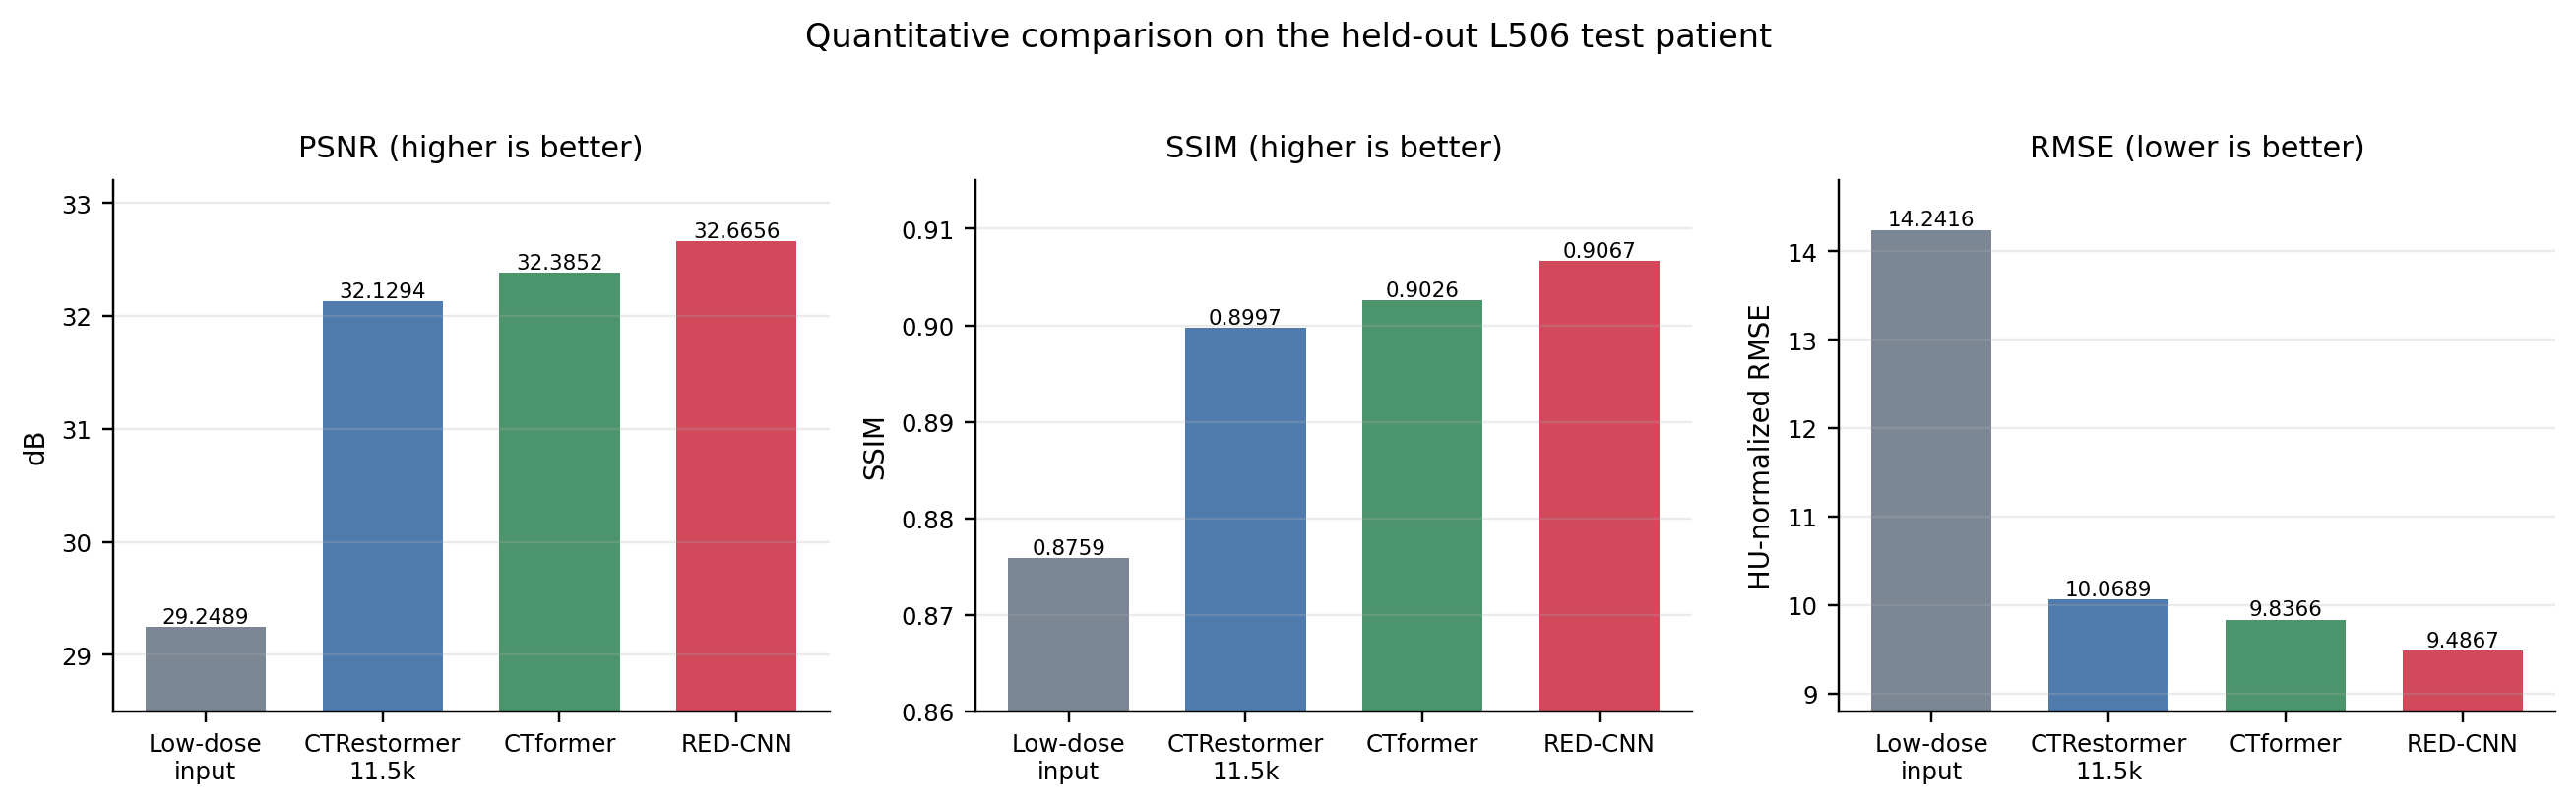
\includegraphics[width=0.9\textwidth]{figures/metrics_comparison.png}
\caption{Metric comparison of low-dose input and denoising models on the held-out L506 patient.}
\label{fig:metrics_comparison}
\end{figure}

\begin{figure}[htbp]
\centering
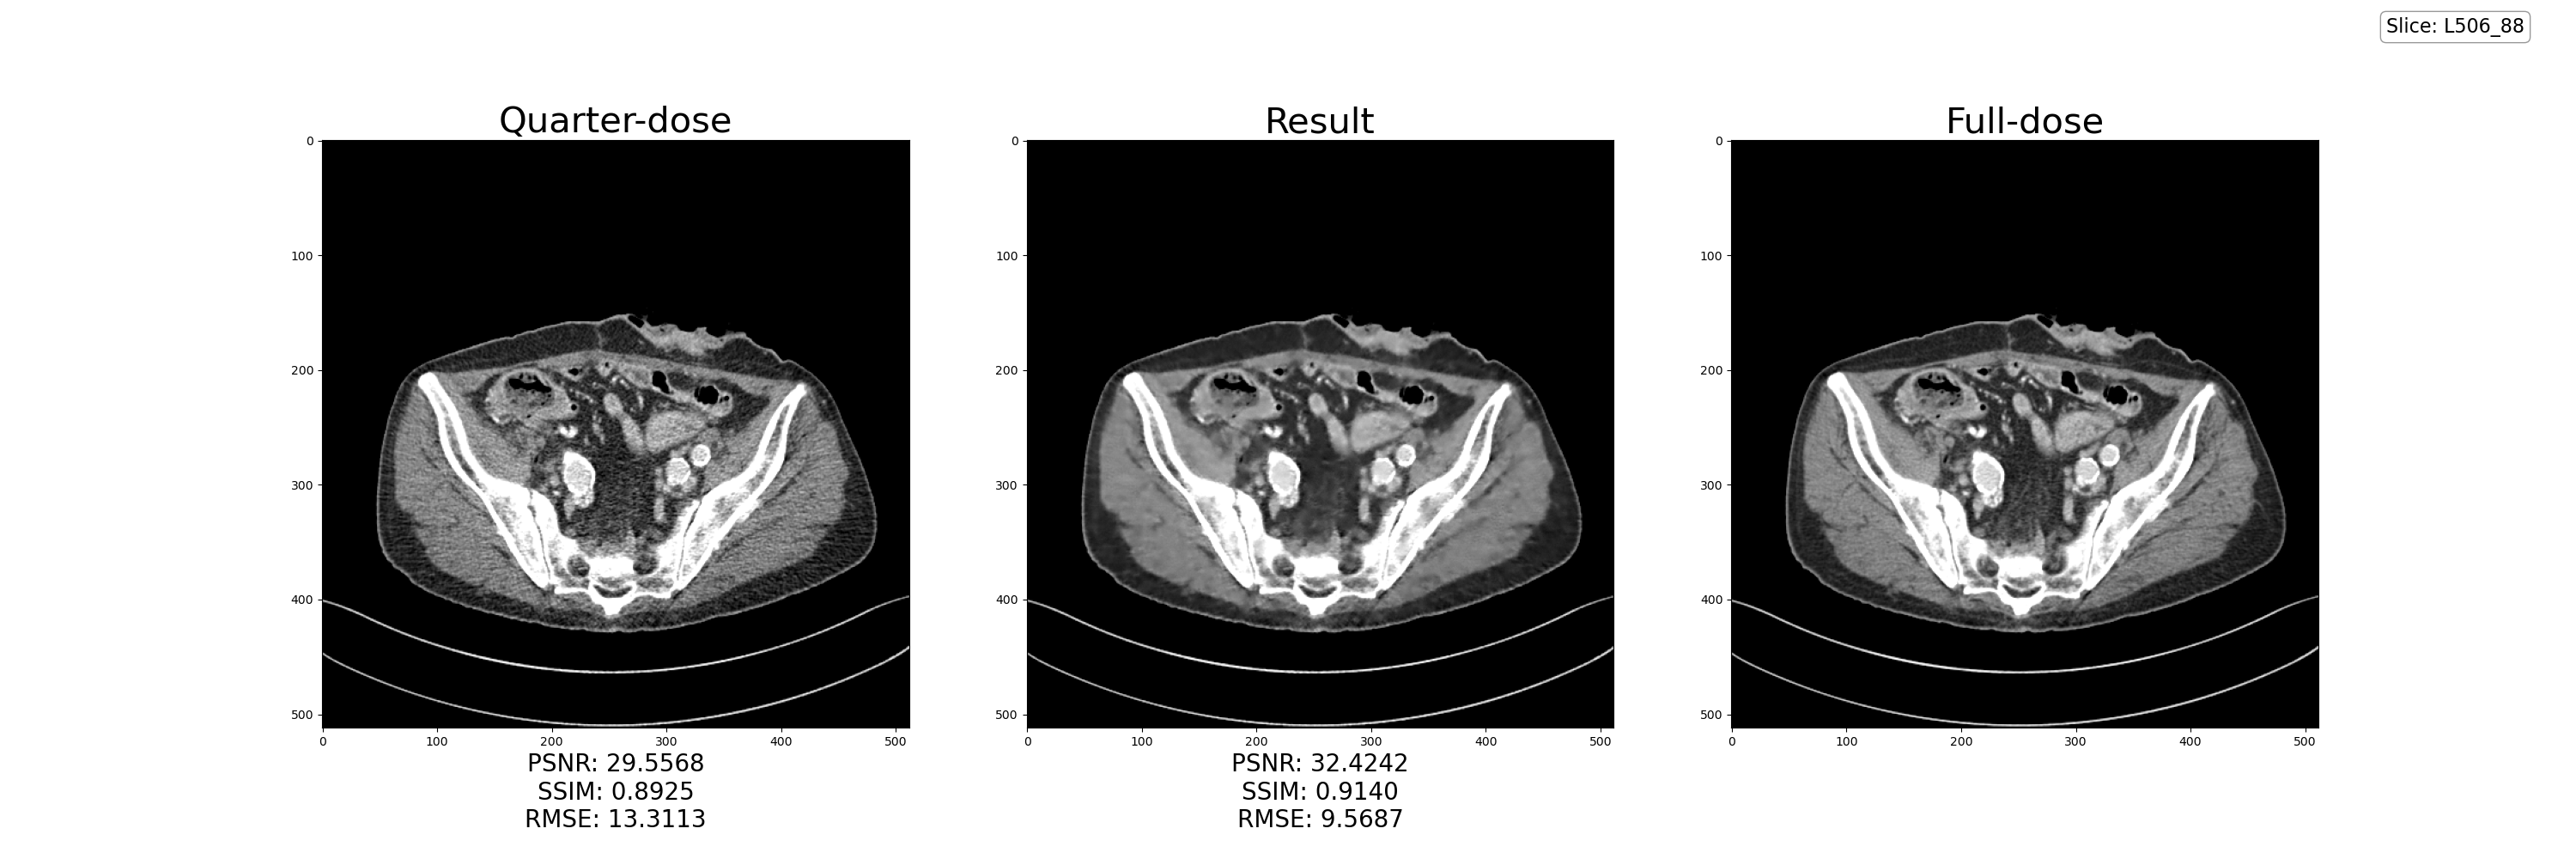
\includegraphics[width=0.95\textwidth]{figures/qualitative_l506_88_ctformer.png}
\caption{Representative qualitative result for slice L506\_88. The denoised image reduces visible noise compared with the low-dose input and approaches the full-dose reference.}
\label{fig:qualitative_ctformer}
\end{figure}

Qualitative inspection is necessary because a model can improve numerical scores while making the image overly smooth. The next important visual extension is to generate residual noise panels containing \(x-y\), \(x-\hat{y}_{RED}\), \(x-\hat{y}_{CTformer}\), and \(x-\hat{y}_{CTRestormer}\). These panels will show whether different models remove similar noise patterns or whether some models remove anatomical edges.

\section{Training Trend}

The CTformer loss curve in Figure \ref{fig:loss_curve} shows convergence during training. A similar loss analysis is useful for CTRestormer, but the more important result is that test metrics continue to change even after the training loss appears plateau-like. This confirms that training loss alone is not enough for checkpoint selection.

\begin{figure}[htbp]
\centering
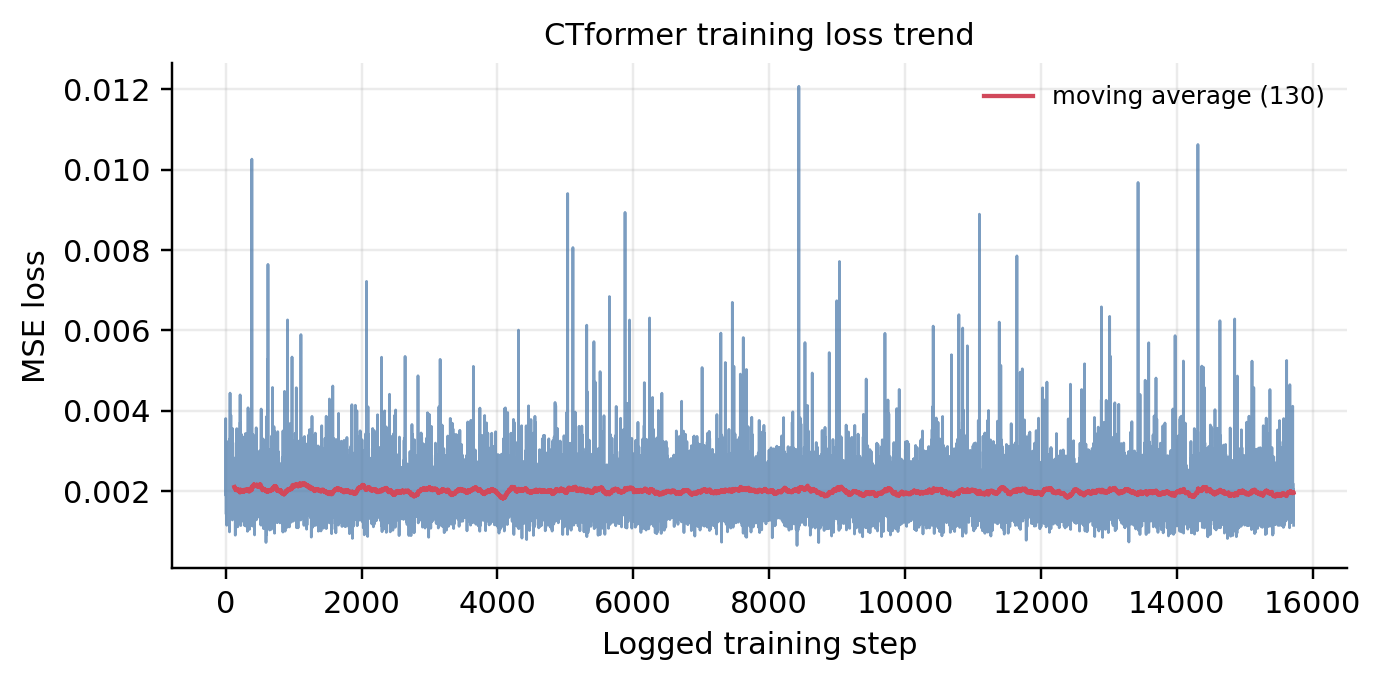
\includegraphics[width=0.75\textwidth]{figures/ctformer_loss_curve.png}
\caption{Training loss trend from the reproduced CTformer run.}
\label{fig:loss_curve}
\end{figure}

\chapter{Discussion and Extended Experiments}

\section{Interpretation of Current Results}

The experiments support three main findings. First, supervised learning is effective for the prepared LDCT dataset. Every learned denoising model improves PSNR, SSIM, and RMSE compared with the low-dose input. Second, CNN baselines remain strong. RED-CNN performs very well because convolution has a strong local inductive bias that matches CT noise removal. Third, the Restormer-style Transformer model becomes competitive only after careful fine-tuning. Its final 21,500-iteration checkpoint slightly exceeds the reproduced baselines, but the margin is small enough that residual analysis is needed before making a strong clinical claim.

The result also highlights a broader lesson: Transformer models are not automatically better than CNNs. Their advantage depends on sufficient training, appropriate model size, stable loss functions, and careful inference. In this project, tiled inference is necessary for CTRestormer because full-image attention would exceed the memory of the available GPU. This is a practical limitation of attention-based restoration models.

\section{Residual Noise Comparison}

The most useful next experiment is residual noise comparison. For each test slice, four maps should be generated:
\[
x-y,\quad x-\hat{y}_{RED-CNN},\quad x-\hat{y}_{CTformer},\quad x-\hat{y}_{CTRestormer}.
\]
If a model is behaving ideally, the removed component should resemble the low-dose noise residual \(x-y\), but should not contain clear anatomical boundaries. If the removed map shows organ edges, bone boundaries, vessels, or lesion-like structures, the model may be suppressing real anatomy.

This experiment can add substantial thesis value because it moves beyond standard metrics. The paper can include a visual panel, histograms, and frequency-domain plots. It can also report correlation between removed residuals and the target edge map:
\begin{equation}
\rho_m = corr(|\nabla y|, |\nabla \hat{n}_m|).
\end{equation}
A lower \(\rho_m\) suggests less anatomical edge leakage into the removed component, although the measure must be interpreted carefully.

\section{Noise Texture and Frequency Analysis}

CT noise has a characteristic texture. A model that removes too much high-frequency content may produce high PSNR but unnatural images. Therefore, noise power spectrum analysis can be added. For each residual map, the two-dimensional Fourier power spectrum is computed and radially averaged. This gives a curve showing how much residual energy exists at different spatial frequencies.

This analysis can compare whether RED-CNN, CTformer, and CTRestormer remove similar frequency bands. For example, a CNN may remove more local high-frequency noise, while a Transformer may also suppress broader low-frequency artifacts. If CTRestormer removes more mid-frequency anatomical texture than the baselines, that would be a warning sign even if its PSNR is high.

\section{Noise2Noise Experiment}

A Noise2Noise-style experiment is attractive, but the current dataset limitation must be handled honestly. The prepared data contains paired quarter-dose and full-dose images, not two independent low-dose acquisitions of the same slice. Therefore, a direct clinical Noise2Noise experiment cannot be claimed unless such pairs are obtained.

A feasible controlled experiment is pseudo Noise2Noise. Starting from full-dose images, two independent synthetic noise realizations can be generated:
\[
x_1 = y + \epsilon_1,\quad x_2 = y + \epsilon_2,
\]
where \(\epsilon_1\) and \(\epsilon_2\) are independent simulated CT-like noise terms. A model is trained to map \(x_1\) to \(x_2\), and then evaluated against the original full-dose \(y\). This can test whether CTRestormer can learn denoising without clean targets under controlled assumptions. The limitation is that synthetic noise may not match real CT acquisition noise.

\section{Other Recommended Extensions}

Several additional experiments can strengthen the final thesis:

\begin{enumerate}[leftmargin=*]
\item \textbf{Loss ablation:} compare MSE, Charbonnier, SSIM, and hybrid loss on the same CTRestormer architecture.
\item \textbf{Checkpoint study:} evaluate 11,500, 16,500, 18,000, 21,500, and 22,000 iterations to determine whether 21,500 is stable or only a lucky checkpoint.
\item \textbf{ROI analysis:} compute PSNR/RMSE separately in air, soft tissue, and bone masks based on CT intensity thresholds.
\item \textbf{Edge preservation:} compare gradient magnitude error and edge maps between denoised outputs and full-dose targets.
\item \textbf{Data expansion:} pretrain on mixed 1mm and 3mm data, then fine-tune on 3mm only, while keeping the same L506 test split.
\item \textbf{Efficiency comparison:} report model parameters, inference time, and GPU memory usage for RED-CNN, CTformer, and CTRestormer.
\item \textbf{Qualitative failure cases:} select slices where CTRestormer improves and slices where it fails, then discuss possible reasons.
\end{enumerate}

Among these, residual noise maps and checkpoint study should be prioritized because they can be completed using the outputs already generated by the current pipeline. Noise2Noise is interesting but should be treated as a secondary extension unless a clean implementation and enough time are available.

\chapter{Conclusion}

This thesis studies low-dose CT denoising as a medical image restoration problem. Using the prepared AAPM-Mayo 3mm B30 dataset and a patient-level held-out test split, it compares low-dose input, RED-CNN, CTformer, and a Restormer-style CTRestormer model. The results show that learned denoising substantially improves over the low-dose input. After fine-tuning, CTRestormer at 21,500 iterations achieves the best current metrics, with 32.6738 dB PSNR, 0.9096 SSIM, and 9.4842 RMSE on the held-out L506 patient.

The findings suggest that Transformer-based restoration is promising for LDCT denoising, but its advantage depends on careful training and evaluation. CNN baselines remain strong, and numerical metrics alone cannot prove clinical quality. The next step is to analyze residual noise maps, noise texture, and edge preservation to determine whether the best model removes noise while preserving true anatomy. This direction will make the final thesis stronger because it connects model performance with medical image reliability rather than relying only on PSNR and SSIM.

\clearpage
\addcontentsline{toc}{chapter}{References}
\begin{thebibliography}{99}
\singlespacing

\bibitem{aapm2016}
American Association of Physicists in Medicine. Low Dose CT Grand Challenge, 2016. Available: \url{https://www.aapm.org/GrandChallenge/LowDoseCT/}.

\bibitem{ronneberger2015}
O. Ronneberger, P. Fischer, and T. Brox, ``U-Net: Convolutional networks for biomedical image segmentation,'' in \textit{Medical Image Computing and Computer-Assisted Intervention}, 2015, pp. 234--241.

\bibitem{chen2017}
H. Chen, Y. Zhang, M. K. Kalra, F. Lin, Y. Chen, P. Liao, J. Zhou, and G. Wang, ``Low-dose CT with a residual encoder-decoder convolutional neural network,'' \textit{IEEE Transactions on Medical Imaging}, vol. 36, no. 12, pp. 2524--2535, 2017.

\bibitem{liang2021}
J. Liang, J. Cao, G. Sun, K. Zhang, L. Van Gool, and R. Timofte, ``SwinIR: Image restoration using Swin Transformer,'' in \textit{Proc. IEEE/CVF International Conference on Computer Vision Workshops}, 2021, pp. 1833--1844.

\bibitem{zamir2022}
S. W. Zamir, A. Arora, S. Khan, M. Hayat, F. S. Khan, M.-H. Yang, and L. Shao, ``Restormer: Efficient Transformer for high-resolution image restoration,'' in \textit{Proc. IEEE/CVF Conference on Computer Vision and Pattern Recognition}, 2022, pp. 5728--5739.

\bibitem{wang2022}
Z. Wang, X. Cun, J. Bao, W. Zhou, J. Liu, and H. Li, ``Uformer: A general U-shaped Transformer for image restoration,'' in \textit{Proc. IEEE/CVF Conference on Computer Vision and Pattern Recognition}, 2022, pp. 17683--17693.

\bibitem{wang2023}
D. Wang, F. Fan, Z. Wu, R. Liu, F. Wang, and H. Yu, ``CTformer: Convolution-free Token2Token dilated vision Transformer for low-dose CT denoising,'' \textit{Physics in Medicine \& Biology}, vol. 68, no. 6, 2023.

\bibitem{lehtinen2018}
J. Lehtinen, J. Munkberg, J. Hasselgren, S. Laine, T. Karras, M. Aittala, and T. Aila, ``Noise2Noise: Learning image restoration without clean data,'' in \textit{Proc. International Conference on Machine Learning}, 2018.

\end{thebibliography}
\doublespacing

\appendix
\chapter*{Appendix}
\addcontentsline{toc}{chapter}{Appendix}

Additional training logs, generated figures, model configuration files, and experiment scripts can be attached here in the final version.

\fronttitle{Author's Biography}
\onehalfspacing

\begin{enumerate}[leftmargin=*,label=\arabic*.]
\item \textbf{Personal Information}

Name: \StudentName

Gender:

Date of Birth:

\item \textbf{Education}

YYYY.MM--YYYY.MM \quad Institution, Degree

\item \textbf{Awards}

\item \textbf{Research Experience}

\item \textbf{Publications and Patents}
\end{enumerate}
\doublespacing

\end{document}
